\documentclass[aspectratio=169]{beamer}

\usepackage{ccicons}
\usepackage{fontspec}
\usepackage{listings}
\usepackage{tikz}
\usepackage{svg}

\definecolor{uclablue}{RGB}{39,116,174}
\definecolor{uclagold}{RGB}{255,179,0}

\definecolor{ubcorange}{RGB}{158, 66, 37}

\definecolor{cugold}{RGB}{207, 184, 124}
\definecolor{cudarkgray}{RGB}{86, 90, 92}

\definecolor{solarizedred}{RGB}{220, 50, 47}
\definecolor{solarizedblue}{RGB}{38, 139, 210}
\definecolor{solarizedgreen}{RGB}{133, 153, 0}
\definecolor{solarizedpurple}{RGB}{108, 113, 196}
\definecolor{solarizedmagenta}{RGB}{211, 54, 130}

\definecolor{pantone655}{RGB}{0, 42, 92}
\definecolor{pantone7453}{RGB}{123, 164, 217}
\definecolor{pantone633}{RGB}{0, 139, 176}
\definecolor{pantone7492}{RGB}{218, 229, 205}

\colorlet{primarycolor}{pantone655}
\colorlet{secondarycolor}{pantone7453}


\usetikzlibrary{
  arrows,
  arrows.meta,
  automata,
  backgrounds,
  calc,
  chains,
  decorations.pathreplacing,
  fit,
  intersections,
  matrix,
  overlay-beamer-styles,
  positioning,
  shapes,
  shapes.multipart,
  tikzmark,
}
\usetikzmarklibrary{listings}

\hypersetup{
  colorlinks=true,
  urlcolor=cudarkgray,
}

\setbeamercolor{frametitle}{fg=primarycolor}
\setbeamercolor{structure}{fg=primarycolor}
\setbeamercolor{enumerate item}{fg=black}
\setbeamercolor{itemize item}{fg=black}
\setbeamercolor{itemize subitem}{fg=black}

\setbeamersize{text margin left=26.6mm}
\addtolength{\headsep}{2mm}

\setbeamertemplate{navigation symbols}{}
\setbeamertemplate{headline}{}
\setbeamertemplate{footline}{}
\setbeamertemplate{itemize item}{\color{black}}
\setbeamertemplate{itemize items}[circle]

\setbeamertemplate{footline}{
  \begin{tikzpicture}[remember picture,
                      overlay,
                      shift={(current page.south west)}]
    \node [black!50, inner sep=2mm, anchor=south east]
          at (current page.south east) {\footnotesize \insertframenumber};
  \end{tikzpicture}
}

\setsansfont{Inter}[Scale=MatchLowercase]
\setmonofont{Hack}[Scale=MatchLowercase]

\makeatletter
\newcommand\version[1]{\renewcommand\@version{#1}}
\newcommand\@version{}
\def\insertversion{\@version}

\newcommand\lecturenumber[1]{\renewcommand\@lecturenumber{#1}}
\newcommand\@lecturenumber{}
\def\insertlecturenumber{\@lecturenumber}
\makeatother

\setbeamertemplate{title page}
{
  \begin{tikzpicture}[remember picture,
                      overlay,
                      shift={(current page.south west)},
                      background rectangle/.style={fill=pantone655},
                      show background rectangle]
    \node [anchor=west, align=left, inner sep=0, text=white]
          (lecturenumber) at (\paperwidth / 6, \paperheight * 3 / 4)
          {\Large Lecture \insertlecturenumber};
    \node [inner sep=0, align=left, text=white, node distance=0,
          above left=of lecturenumber, anchor=south west, yshift=2mm]
          {\Large ECE 344: Operating Systems};
    \node (title) [inner sep=0, anchor=west, align=left, text=white,
                   text width=30em]
          at (\paperwidth / 6, \paperheight / 2)
          {{\bfseries \Huge \inserttitle{}}};
    \node [inner sep=0, align=right, text=white, node distance=0,
          below right=of title, anchor=north east, yshift=-1mm]
          {{\footnotesize \ttfamily \insertversion}};
    \node [inner sep=0, text=white, align=left, anchor=west]
          (author) at (\paperwidth / 6, \paperheight / 4)
          {\insertauthor};
    \node [text=white, inner sep=0, align=left, node distance=0,
           below left=of author, anchor=north west, yshift=-2mm]
          {\insertdate};
    \node [align=right, anchor=south east, inner sep=2mm, text=white]
          (license) at (\paperwidth, 0)
          {\footnotesize This  work is licensed under a
           \href{http://creativecommons.org/licenses/by-sa/4.0/}
                {\color{pantone7453} Creative Commons Attribution-ShareAlike 4.0
                 International License}};
    \node [text=white, inner sep=0, align=right, node distance=0,
           above right=of license, anchor=south east, xshift=-2mm]
          {\Large \ccbysa};
  \end{tikzpicture}
}

\tikzset{
  >=Straight Barb[],
  shorten >=1pt,
  initial text=,
}

\lstset{
  basicstyle=\footnotesize\ttfamily,
  language=C,
  escapechar=@,
  commentstyle=\color{black!50},
}


\lecturenumber{20}
\title{Multi-Level Page Tables}
\version{1.0.0}
\author{Jon Eyolfson}
\date{October 25/26, 2021}

\begin{document}
  \begin{frame}[plain, noframenumbering]
    \titlepage
  \end{frame}

  \begin{frame}
    \frametitle{Multi-Level Page Tables Save Space for Sparse Allocations}

    \begin{center}
      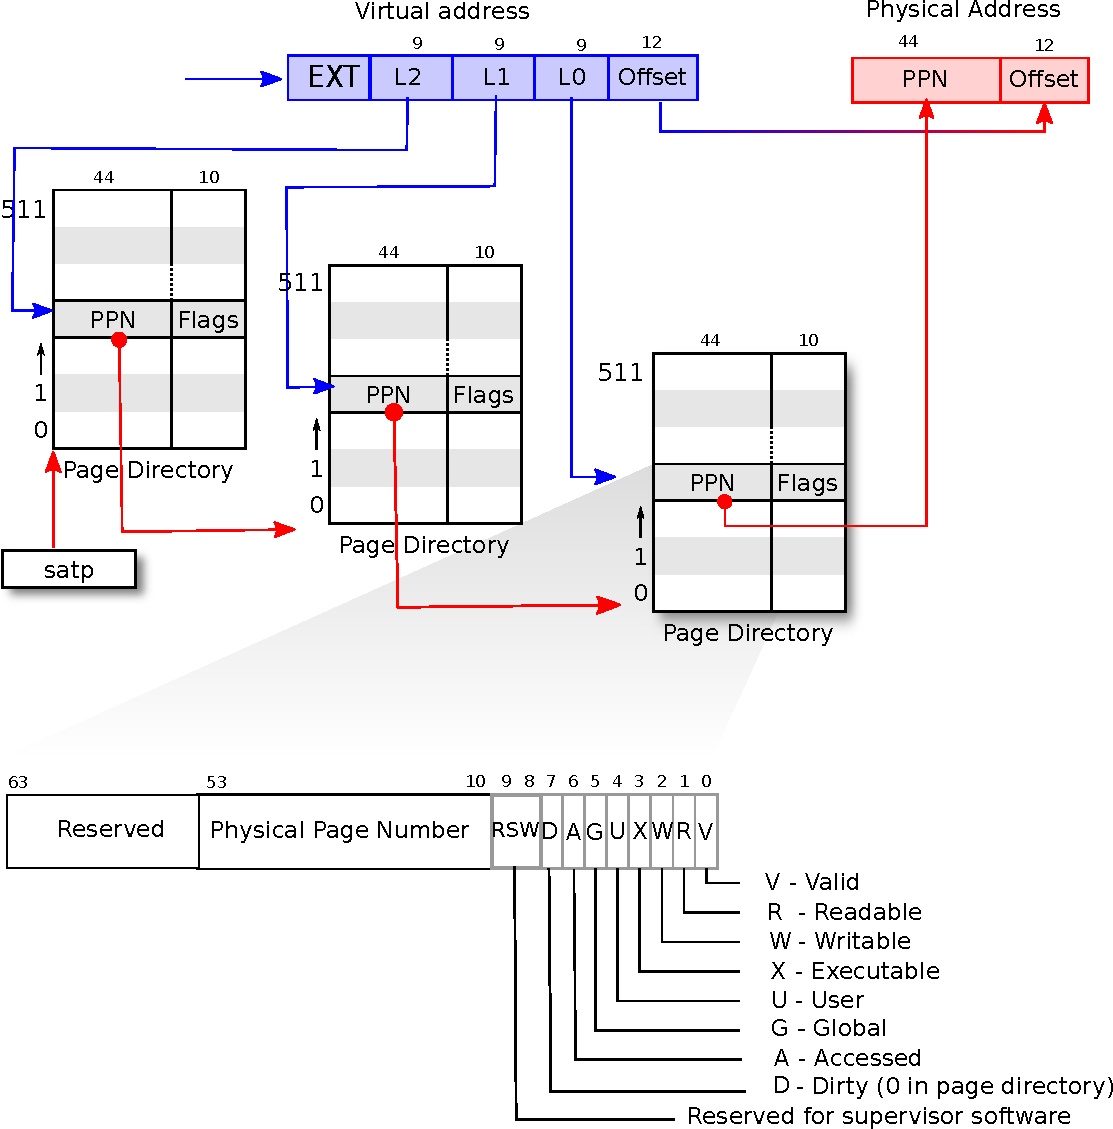
\includegraphics[scale=0.5, clip, trim=0cm 8cm 0cm 0cm]{../lecture-19/riscv_pagetable.pdf}
    \end{center}

    © MIT \url{https://github.com/mit-pdos/xv6-riscv-book/}
  \end{frame}

  \begin{frame}
    \frametitle{For RISC-V Each Level Occupies One Page}

    There are 512 ($\mathsf{2^9}$) entries of 8 bytes($\mathsf{2^3}$) each, which is 4096 bytes

    \vspace{2em}

    The PTE for L(N) points to the page table for L(N-1)

    \vspace{2em}

    You follow these page tables until L0 and that contains the \texttt{PPN}
  \end{frame}

  \begin{frame}
    \frametitle{Consider Just One Additional Level}

    Assume our process uses just one virtual address at \texttt{0x3FFFF008}

    \hspace{2em} or \texttt{0b11\_1111\_1111\_1111\_1111\_0000\_0000\_1000}

    \hspace{2em} or \texttt{0b111111111\_111111111\_000000001000}

    \vspace{2em}

    We'll just consider a 30-bit virtual address with a page size of 4096 bytes

    \hspace{2em} We would need a 2 MiB page table if we only had one ($\mathsf{2^{18} \times 2^{3}}$)

    \vspace{2em}

    Instead we have a 4 KiB L1 page table ($\mathsf{2^9 \times 2^{3}}$) and a 4 KiB L0 page table

    \hspace{2em} Total of 8 KiB instead of 2 MiB

    \vspace{2em}

    Note: worst case if we used all virtual addresses we would consume 2 MiB + 4 KiB
  \end{frame}

  \begin{frame}
    \frametitle{Translating \texttt{3FFFF008} with 2 Page Tables}

    Consider the L1 table with the entry:

    \begin{center}
    {\ttfamily
    \begin{tabular}{rl}
      Index & PPN \\
      511   & 0x8 \\
    \end{tabular}}
    \end{center}
      
    Consider the L0 table located at \texttt{0x8000} with the entry:

    \begin{center}
    {\ttfamily
    \begin{tabular}{rl}
      Index & PPN \\
      511   & 0xCAFE \\
    \end{tabular}}
    \end{center}
    
    The final translated physical address would be: \texttt{0xCAFE008}
  \end{frame}

  \begin{frame}
    \frametitle{Processes Use A Register Like \texttt{satp} to Set the Root Page Table}

    \begin{center}
      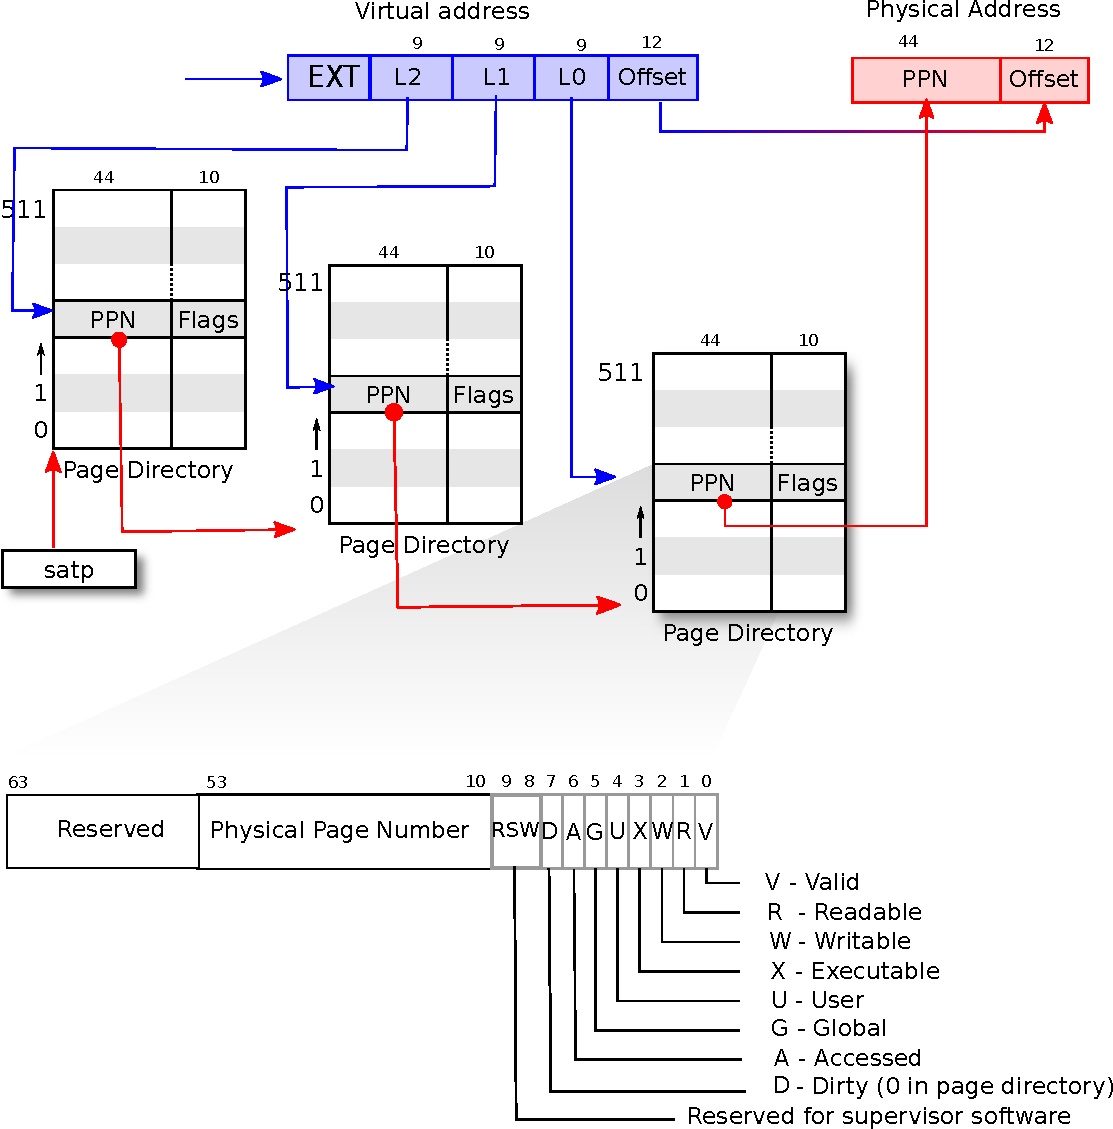
\includegraphics[scale=0.5, clip, trim=0cm 8cm 0cm 0cm]{../lecture-19/riscv_pagetable.pdf}
    \end{center}

    © MIT \url{https://github.com/mit-pdos/xv6-riscv-book/}
  \end{frame}

  \begin{frame}
    \frametitle{Page Allocation Uses A Free List}

    Given physical pages, the operating system maintains a free list (linked list)

    \vspace{2em}

    The unused pages themselves contain the \texttt{next} pointer in the free list

    \hspace{2em} Physical memory gets initialized at boot

    \vspace{2em}

    To allocate a page, you remove it from the free list

    \hspace{2em} To deallocate a page you add it back to the free list
  \end{frame}

  \begin{frame}
    \frametitle{Using the Page Tables for Every Memory Access is Slow}

    We need to follow pointers across multiple levels of page tables!

    \vspace{2em}

    We'll likely access the same page multiple times (close to the first access time)

    \vspace{2em}

    A process may only need a few VPN $\rightarrow$ PPN mappings at a time

    \vspace{2em}

    Our solution is another computer science classic: caching
  \end{frame}

  \begin{frame}
    \frametitle{A Translation Look-Aside Buffer (TLB) Caches Virtual Addresses}

    \begin{center}
    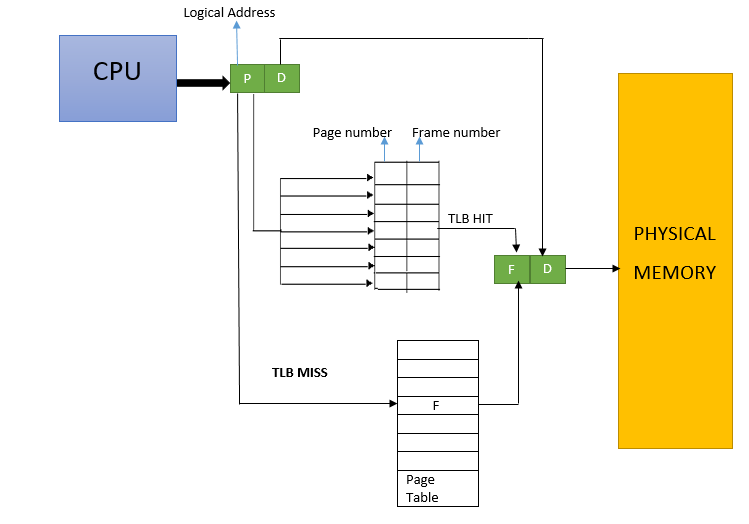
\includegraphics[scale=0.45]{tlb.png}
    \end{center}

    ``Working flow of a TLB'' by Aravind Krishna is licensed under CC BY-SA 4.0
  \end{frame}

  \begin{frame}
    \frametitle{Effective Access Time (EAT)}

    Assume a single page table (there's only one additional memory access in the page table)

    \vspace{2em}

    $\mathsf{TLB\_Hit\_Time = TLB\_Search + Mem}$

    $\mathsf{TLB\_Miss\_Time = TLB\_Search + 2 \times Mem}$

    $\mathsf{EAT = \alpha \times TLB\_Hit\_Time + (1 - \alpha) \times TLB\_Miss\_Time}$

    \vspace{2em}

    If $\mathsf{\alpha = 0.8}$, $\mathsf{TLB\_Search = 10\ ns}$, and memory accesses take 100 ns, calculate EAT

    \hspace{2em} $\mathsf{EAT = 0.8 \times 110\ ns + 0.2 \times 210\ ns}$

    \hspace{2em} $\mathsf{EAT = 130\ ns}$
  \end{frame}

  \begin{frame}
    \frametitle{Context Switches Require Handling the TLB}

    You can either flush the cache, or attach a process ID to the TLB

    \vspace{2em}

    Most implementation just flush the TLB

    \hspace{2em} RISC-V uses a \texttt{sfence.vma} instruction to flush the TLB

    \vspace{2em}

    On x86 loading the base page table will also flush the TLB

  \end{frame}

  \begin{frame}
    \frametitle{How Many Levels Do I Need?}

    Assume we have a 32-bit virtual address with a page size of 4096 bytes

    \hspace{2em} and a PTE size of 4 bytes

    \vspace{2em}

    We want each page table to fit into a single page

    \hspace{2em} Find the number of PTEs we could have in a page ($\mathsf{2^{10}}$)

    \hspace{4em} $\mathsf{log_2(\# PTEs\ per\ Page)}$ is the number of bits to index a page table

    \vspace{2em}

    $\mathsf{\# Levels = \lceil \frac{Virtual\ Bits - Offset\ Bits}{Index\ Bits} \rceil}$

    \vspace{2em}

    \onslide<2->{$\mathsf{\# Levels = \lceil \frac{32 - 12}{10} \rceil = 2}$}
  \end{frame}

  \begin{frame}[fragile]
    \frametitle{TLB Testing}

    Check out \texttt{lecture-08/test-tlb}

    \hspace{2em} (you may need to \texttt{git submodule update --init --recursive})

    \vspace{2em}

    \texttt{./test-tlb <size> <stride>}

    \hspace{2em} Creates a <size> memory allocation and acccesses it every <stride> bytes

    \vspace{2em}

    Results from my laptop:

    \begin{lstlisting}
> ./test-tlb 4096 4        
  1.93ns (~7.5 cycles)
> ./test-tlb 536870912 4096
155.51ns (~606.5 cycles)
> ./test-tlb 16777216 128  
 14.78ns (~57.6 cycles)
    \end{lstlisting}
  \end{frame}

  \begin{frame}
    \frametitle{Use \texttt{sbrk} for Userspace Allocation}

    This call grows or shrinks your heap (the stack has a set limit)

    \vspace{2em}

    For growing, it'll grab pages from the free list to fulfill the request

    \hspace{2em} The kernel sets \texttt{PTE\_V} (valid) and other permissions

    \vspace{2em}

    In memory allocators this is difficult to use, you'll rarely shrink the heap

    \hspace{2em} It'll stay claimed by the process, and the kernel cannot free
    pages

    \vspace{2em}

    Memory allocators use \texttt{mmap} to bring in large blocks of virtual
    memory
  \end{frame}

  \begin{frame}
    \frametitle{The Kernel Initializes the Processs' Address Space (and Stack)}

    \begin{center}
      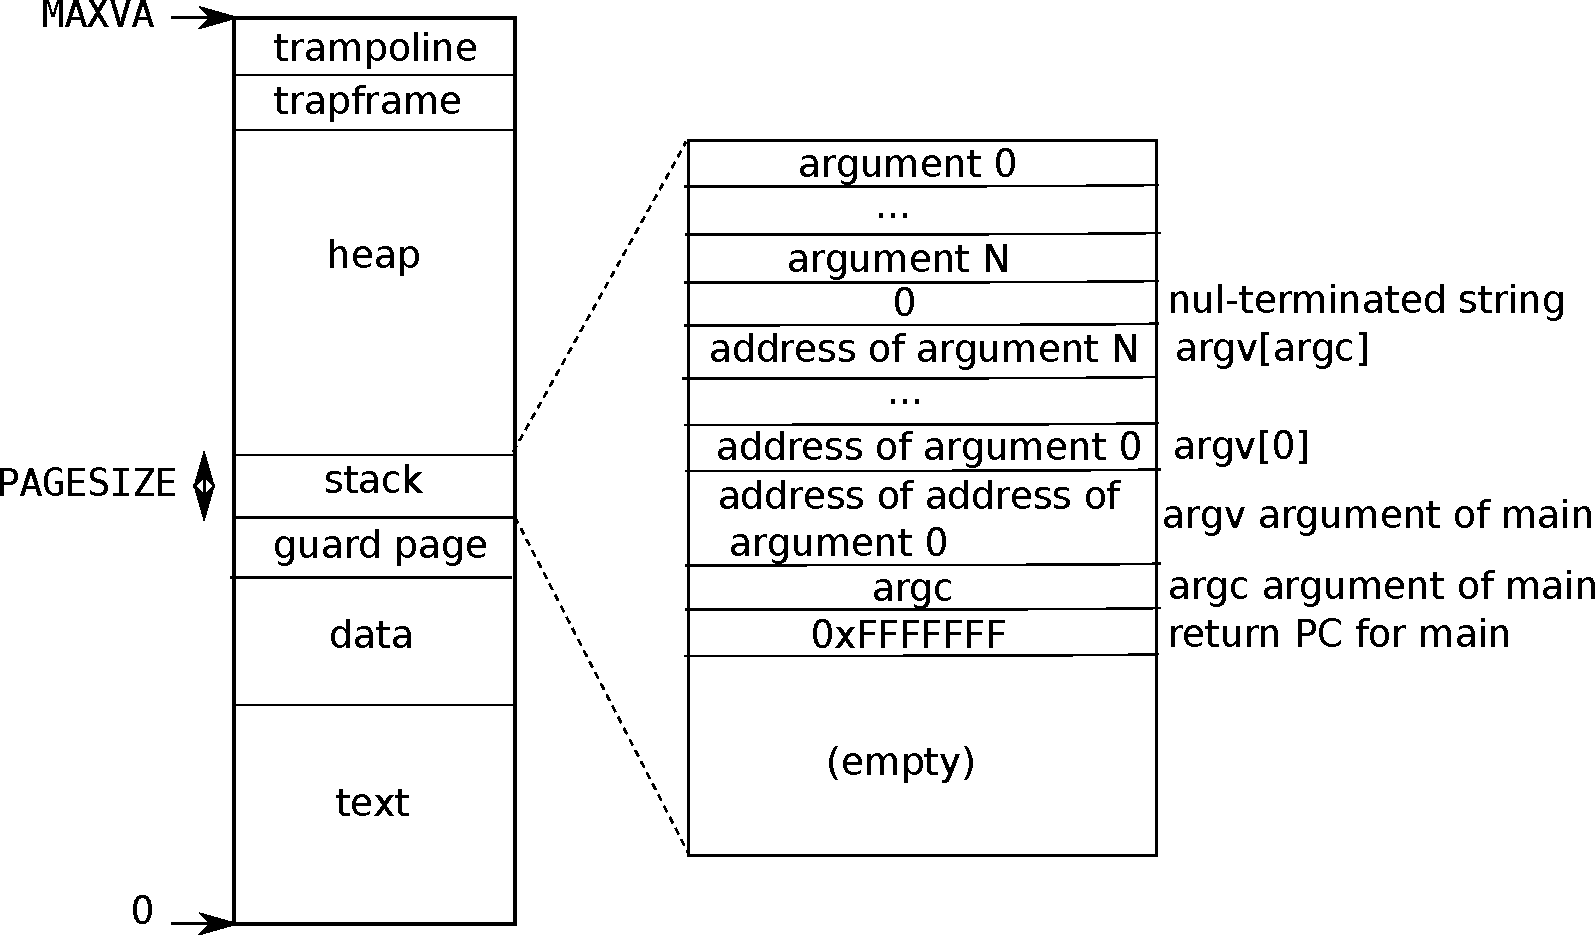
\includegraphics[scale=0.35]{processlayout.pdf}
    \end{center}

    © MIT \url{https://github.com/mit-pdos/xv6-riscv-book/}
  \end{frame}

  \begin{frame}
    \frametitle{A Trampoline is A Fixed Virtual Address Set by the Kernel}

    It allows the process to access kernel data without using
    a system call

    \vspace{2em}

    The guard page will generate an exception if accessed meaning stack overflow

    \vspace{2em}

    A trap is anytime special handler code runs:
    \begin{itemize}
      \item System call
      \item Exception
      \item Interrupt (e.g timer)
    \end{itemize}
  \end{frame}

  \begin{frame}
    \frametitle{Page Faults Allow the Operating System to Handle Virtual Memory}

    Page faults are a type of exception for virtual memory access

    \hspace{2em} Generated if it cannot find a translation, or permission check fails

    \vspace{2em}

    This allows the operating system to handle it

    \hspace{2em} We could lazily allocate pages, implement copy-on-write, or swap to disk
  \end{frame}

  \begin{frame}
    \frametitle{Page Tables Translate Virtual to Physical Addresses}

    The MMU is the hardware that uses page tables, which may:
    \begin{itemize}
      \item Be a single large table (wasteful, even for 32-bit machines)
      \item Be a multi-level to save space for sparse allocations
      \item Use the kernel allocate pages from a free list
      \item Use a TLB to speed up memory accesses
    \end{itemize}
  \end{frame}
\end{document}
